\chapter{Reinforcement-Learned Stabilisation}
\label{chap:rl_walk}

\section{Introduction}

A major goal of the RoboCup Standard Platform League is the development of improved bipedal control of the Nao robots. The teams aim to demonstrate that the robots are able to execute increasingly human-like bipedal behaviours, whether it be walking, kicking a ball, or self-stabilisation. The ability to execute these types of movements, to be able to switch between them fluidly, and to react against external forces to avoid falling over is a key research area in robotics. The responsiveness required by such movements is what is to be expected of future robots particularly when emulating human behaviours, as in playing a game of soccer.

Such behaviour is extremely difficult or practically impossible to be programmed directly into a robot. Careful study and analysis of human movement is required and mathematical models must be derived to approximate it. Even then, such models tend only to work in ideal situations, such as walking over a perfectly smooth and flat ground. In order to approach the behaviour that is inherent in humans -- that of adapting to any possible situation -- it is necessary that machine-learning principles are considered in order to adapt to any change in the robot's environment. For example, a hand-programmed walk will react differently over a rough and bumpy surface than over a flat and smooth surface, as it is confined to a small subset of possible robot states, whereas a machine-learned walk should in theory be able to react to either.

For the 2013 Open Challenge, we explored the application of Reinforcement-Learned behaviours for bipedal movements on the Nao robots. We aimed to demonstrate that simulator-learned behaviours could be applied directly to the Nao robots without the need for significant tuning in software. The Open Challenge entry was titled \textit{``Stability Control through Machine Learned Behaviours''}\cite{openchallenge}.

The learned behaviours aimed to react to a greater number of states than hand-programming would allow for and to allow relatively simpler implementation of more advanced behaviours. Applied to the Naos, we aimed for self-stabilisation without the need for hard-coding in a variety of states including: changing support feet at different frequencies (walking on the spot); standing upright; standing on either foot; and seamlessly switching between these. 

\newpage
\section{Background \& Related Work}

Reinforcement Learning (RL) is a method of deriving software models for behaviour through machine learning. RL is used to automatically determine a model for actions to be taken given an \textit{environment state} such that the maximum \textit{reward} can be achieved. In the context of stability control for bipedal robots, RL results in a software model (known as a \textit{policy}) which states what motors the robot should actuate and in what manner, given that the robot is in some state (the environment state) and wants to reach some position (the reward).

An RL model is defined by:\cite{bernhard_rl}

\begin{description}
\item[States] -- the set of all states the robot can be expected to act in.
\item[Actions] -- the set of all actions the robot can potentially take.
\item[Transitions] -- the definition of how states transition into other states.
\item[Reward] -- the definition of how good being in a certain state or doing a certain action is.
\end{description}

%The Q-learning -> learns to assign values to (s,a) pairs.
%Given a particular action in a particular state, followed by actions which follow a particular policy, the agent will receive a particular set of reinforcement.

RL works by finding a function which gives the value of taking a particular action when in a particular state and then following the optimal policy thereafter. The optimal value is therefore the best one of the possible actions that can be taken at a given state. The \textit{value} of each state-action is dependent on the reward -- taking actions which lead to rewards quickly is of higher value, taking actions which lead to slow or negative rewards is of lower value.

The work presented in this report relies primarily on the application of RL research done by Hengst\cite{bernhard_rl}. Hengst's work involved the use of a simulated environment for the robot, allowing for fast reinforcement learning of optimal policies for various behaviours (defined by their cost (inverse of reward) functions), including:

\begin{itemize}
\item Standing upright and still.
\item Standing on one leg.
\item Rocking between both legs.
\end{itemize}

Hengst's work allows for a much simpler implementation of the policies in real hardware with less need for learning or tuning on the hardware. Testing this is one of the primary aims of the work outlined in this report.

White's\cite{white} 2011 implementation of a simulator-learned policy for a walking gait on the Naos is also an important motivator. White was able to show that a simulator-learned walk running on the Naos was able to react to obstacles significantly better than one with no RL policy. However, White also found that state measurement was very difficult due to noisy sensors and limited data, and the work was not merged into the competition code.

Further work by Liu\cite{liu} in 2012 focused primarily on improving state measurement by introducing heavy filtering of the Inertial Measurement Unit (IMU) located in the chest of the Naos. While the demonstrated filters worked well, Liu found that the underlying assumptions in the filter (that the robot is standing still, upright, and approximates an inverted pendulum) were not sufficient when introducing more complex motion such as a walking gait.

\newpage
\section{Theory \& Implementation}

The work presented involves an attempt to combine the previous works of Hengst, White, and Liu in order to produce these self-stabilising behaviours, and to explore the application to walk stabilisation. Below we detail the theory and implementation of the major aspects of this work, which include: learning the control policies, measuring the current state, and interpreting the policies in the software.

\subsection{Learning the Control Policies}
\label{sec:learning_policies}
In learning the policies for the behaviours, Hengst\cite{bernhard_rl} defines a robot model, including as much accuracy in the links, joints, masses, etc. as possible -- an example of this is seen in Figure~\ref{fig:lean}.

\begin{figure}[h]
\centering
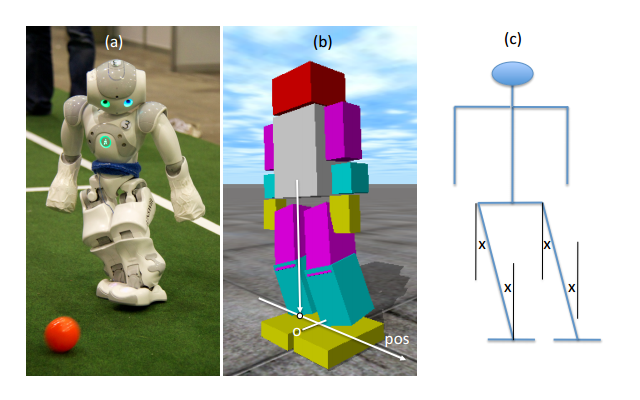
\includegraphics[width=3.5in]{img/RL_lean.png}
\vspace{-10pt}
\caption{The Nao robots modelled as a $23 DOF$ (Degree of Freedom) system in (b). \cite{bernhard_rl}}
\label{fig:lean}
\end{figure}

Hengst defines the \textit{state} of the robot using two variables:
\begin{itemize}
\item position of the middle of the torso in $m$eters
\item velocity of the middle of the torso in $\sfrac{m}{s}$
\end{itemize}

The goal or reward function of a behaviour is therefore based on getting to some state (as in standing still) or reaching some states at a certain time (as in rocking back and forth). Example policies can be seen in Figure~\ref{fig:policy_diagram}.

\begin{figure}[!h]
\centering
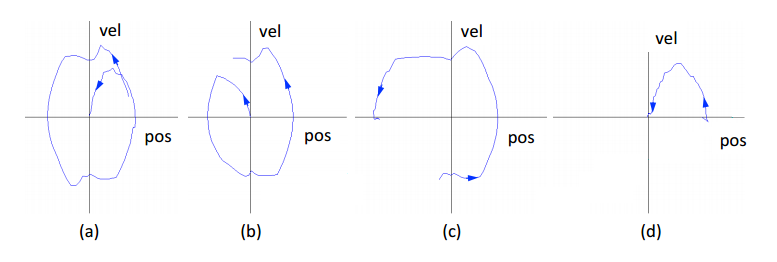
\includegraphics[width=5in]{img/RL_policies.png}
\vspace{-10pt}
\caption{Example of learned policies in the two state variables (position and velocity). The policy defines what actions to take which will lead to the state approaching some goal (for example, zero position and velocity for standing still, as in (a)).\cite{bernhard_rl}}
\label{fig:policy_diagram}
\end{figure}

Knowing how the state of the environment changes based on actions is what the transition function defines. The transition function is calculated by observing the change between states of the simulation when subjected to a random choice of actions (from the set of actions that could be taken) -- the random simulation essentially explores the state space of the model through the actions. This is a computing-intensive process (taking upwards of several hours to complete, depending on the desired resolution) but is also practically impossible to define through real-life hardware testing (due to the complexity in analysing the environment, something a simulation can do very easily).

Once the state transitions are known (to whatever degree), it is a simple case of calculating the value of each state-action for any given reward function, and then finding the optimal action to take for a given state-action (that is to say, the action to take depends not only on the current state, but also on the previous action taken). The list of optimal actions for each state-action is then known as the \textit{optimal policy}. A reward function can be easily created for any goal desired, such as standing still or walking on the spot, so long as the goal states are in the set of explored states. Knowing the state transitions also allows for quick switching between behaviours by simply picking which policy to follow.

A total of 7 goal states were defined: 6 in the coronal plane (side-to-side motions), and 1 in the sagittal plane (front-to-back motions). These goals were as follows:

\begin{enumerate}
\item Standing still
\item Fast pace rocking between feet
\item Medium pace rocking between feet
\item Slow pace rocking between feet
\item Standing on right leg
\item Standing on left leg
\item Sagittal: standing still
\end{enumerate}

The RL process learns the actions required for optimal stabilisation of these goals, and the result can be used to easily transition between the goals by simply following the policy of a new goal. The optimal policies, which define the action required for each possible state, are then defined. Some simplified example policies can be seen earlier in Figure \ref{fig:policy_diagram}.

The optimal policies are then given as a simple output of numbers, being the state-action pair and the corresponding optimal action to take. An example output from a control policy can be seen in Figure~\ref{fig:policy}. This is known as a \textit{policy file}, which can then be interpreted by the robot's software.

\begin{figure}[h]
\newcommand\statehighlight[1]{\textcolor[rgb]{0,1,0}{#1}}
\newcommand\actionhighlight[1]{\textcolor[rgb]{0,0,1}{#1}}
\begin{Verbatim}[commandchars=\\\{\},frame=single]
// Policy table for 6 Coronal behaviours
// State-action is defined by: Goal, lateral torso position, 
//                             lateral torso velocity, last action taken
// Action: 0 for ankle roll left, 1 for none, 2 for ankle roll right
//  \statehighlight{state-action}    \actionhighlight{action}
   0 -0.08 -0.4  0     0
   0 -0.08 -0.39 0     1
   0 -0.08 -0.38 0     1
   0 -0.08 -0.37 0     2
\end{Verbatim}
\vspace{-15pt}
\caption{An excerpt of a control policy for coronal behaviours.}
\label{fig:policy}
\end{figure}

Hengst defines a total of 7 goals, mentioned earlier in this section. These goals and the actions available to the optimal policy calculations are described below:

\subsubsection{Sagittal Goals}
\label{sec:sagittal}

In the sagittal plane, only one goal is defined: standing still and upright.

As described by Hengst\cite{sagittal}, the goal defined for standing still is to return to a state of $(0,0,2)$. This corresponds to returning to a neutral torso position (with no velocity and at a zero position) and then take no action.

As a sagittal policy, we are concerned with movement of the torso in the sagittal plane (in other words, leaning forward or back). The possible actions involve actuating the hip and ankle pitch in order to return the leaning torso to the neutral position. The actions are defined very simply as:

\begin{equation} \label{eq:sagittal}
\delta = 0.01 * (\text{action} - 2)
    \end{equation}

The value of $\delta$ is the \textit{adjustment} in radians added to the hip and ankle pitch angles. We let action be an integer from $0$ to $4$, so that Equation~\ref{eq:sagittal} defines a $\pm0.02$ radians adjustment, $\pm0.01$ radians adjustment, or no adjustment at all (in the case of action $2$) to the motors.

On every tick the current state is defined, the next action is looked up from the policy, and the following occurs:

\begin{lstlisting}
float adjustment = 0.01 * (action - 2);
jointAngle[Joint.LAnklePitch.iD()]  += adjustment;
jointAngle[Joint.RAnklePitch.iD()]  += adjustment;
jointAngle[Joint.LHipPitch.iD()]    += adjustment;
jointAngle[Joint.RHipPitch.iD()]    += adjustment;
\end{lstlisting}

\subsubsection{Coronal Goals}
\label{sec:coronal}

In the coronal plane, six goals are defined. The policies for these goals are a little more complex than for sagittal, so further information should be sought in the technical documentation provided by Hengst.\cite{coronal}

The coronal goals include: standing still, fast, medium, and slow pace rocks from foot to foot, and standing still on either leg.

As some of the goals require a swaying of the robot's hips from side to side to shift the weight between either foot, part of the policy defines a \textit{hip sway} variable as simply a constant multipllied by the current lateral position of the torso.

For the coronal plane, only side-to-side movement is important, so the actions involve actuating the hip and ankle roll motors. The actions are defined as:

\begin{equation} \label{eq:sagittal}
\delta = 0.045 * (\text{action} - 1)
\end{equation}

where $\delta$ is the adjustment in radians, and actions are $0$ to $2$, such that action $1$ means no adjustment.

Again, on every tick the current state is defined, the next action is looked up from the policy, and the behaviour below occurs. It is important to note that some other updates and calculations are also performed depending on which goal is required (for example, lifting up the legs when necessary). Notice that the hip sway adjustment is added to the ankle and hip rolls in opposition to each other.

\begin{lstlisting}
float adjustment  = 0.045 * (action - 1);
float hipSway     = 4 * position;
jointAngle[Joint.LAnkleRoll.iD()] = -hipSway + adjustment;
jointAngle[Joint.RAnkleRoll.iD()] = -hipSway + adjustment;
jointAngle[Joint.LHipRoll.iD()]   = hipSway;
jointAngle[Joint.RHipRoll.iD()]   = hipSway; 
\end{lstlisting}

\subsection{State Measurement on Hardware}

The Nao robots contain an Inertial Measurement Unit (IMU) in their chest, consisting of 2 gyrometers and a three-axis accelerometer.\cite{nao_imu} By knowing the location of the IMU, most importantly its height from the bottom of the feet (dimensions given by Aldebaran Robotics), and ensuring this matches with the simulator, one can use simple trigonometry to calculate the required position and velocity state variables. 

As seen in Figure~\ref{fig:trig}, we can define a simple axis system from the IMU, with the $x$-axis pointing towards the front of the robot, the $y$-axis towards the side, and the $z$-axis pointing down to the ground. This coordinate system applies to the three-axis accelerometer, which provides a $\sfrac{m}{s^2}$ acceleration reading for each of these axes. The accelerometer readings can be used to help calibrate the gyrometer, as the accelerometer should expect to read $9.81\sfrac{m}{s^2}$ for the $z$-axis and $0\sfrac{m}{s^2}$ for the $x$- and $y$-axes when the robot is standing upright and still.

\begin{figure}[h]
\centering
\begin{subfigure}{0.4\textwidth}
  \centering
  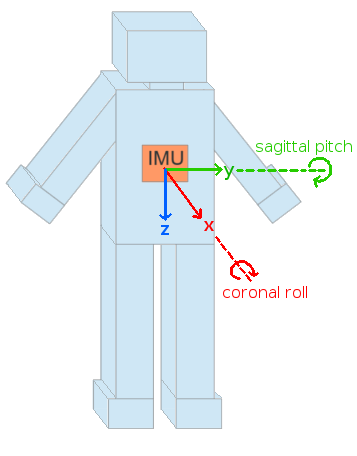
\includegraphics[height=8cm]{img/axes.png}
  \caption{Axes}
  \label{fig:trig}
\end{subfigure}
\begin{subfigure}{0.4\textwidth}
  \centering
  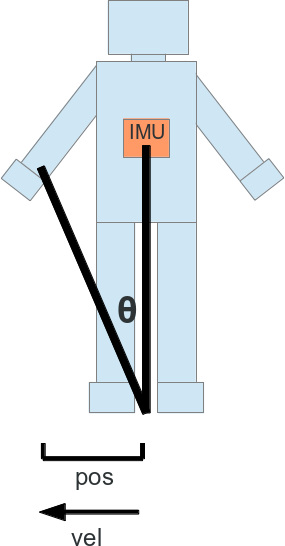
\includegraphics[height=8cm]{img/lean_trig.png}
  \caption{State variables}
  \label{fig:triangle}
\end{subfigure}
\caption{(a) The definition of the $x$-, $y$-, and $z$-axes from the IMU's accelerometers, and the lean angles from the gyrometers.\\(b) The coronal state variables are the lateral position and velocity along the $y$-axis of the IMU in the torso of the Nao robots. $\theta$ is the coronal roll angle given by the gyrometer.}
\label{fig:total}
\end{figure}

The position and velocity of the IMU is taken with respect to its neutral position, when the robot is standing upright. In this way, it is expected that the coronal (side to side) position of the IMU is exactly centered between the two feet. The two gyrometers provide an angular measurement of the torso, being the angle of lean about the $x$-axis (which we shall call the \textit{coronal roll}) and the lean about the $y$-axis (the \textit{sagittal pitch}), as seen in Figure~\ref{fig:trig}. Note that coronal and sagittal refer to the planes dividing a body into front-back and left-right sides respectively. When standing upright the torso is expected to be at a pitch angle of $0\degree$ relative to the hip pitch (which depends on the way the legs are bent while in a standing position), and a roll angle of $0\degree$.

If we assume small perturbations to the torso (in other words, only small pitch and roll angles will be in the state space of the policy), then we can approximate the position of the torso by simply using the gyrometer measurements and the known height of the IMU from the base of the feet. As seen in Figure~\ref{fig:triangle}, which shows a lean in the $x$-axis (or a coronal roll), we can easily calculate the horizontal displacement of the IMU by with: 

\begin{equation} \label{eq:height}
x_t = H * \sin{\theta_t}
\end{equation}

where $x_t$ is the position state variable at time $t$, $H$ is some constant (the height of the IMU), and $\theta_t$ is the angle of the torso lean at time $t$.

Furthermore, for small angles of $|\theta| < 30\degree$, we know that $\sin{\theta} \approx \theta$ (in radians). Thus, we can approximate the lateral position of the IMU by simplifying Equation\ref{eq:height}:

\begin{equation} \label{eq:simplified}
x_t = H\theta_t
\end{equation}

The velocity can be found in one of two ways:
\begin{itemize}
\item Integrate the accelerometer readings in the desired axis over time, or,
\item Differentiate the position readings of the desired axis over time.
\end{itemize}

Both of these are relatively simple to achieve. In theory, integrating the accelerometer readings should provide an accurate velocity at all instants of time. Differentiating the position however means that only the instantaneous velocity is reported, as in:

\begin{equation}
v_t = (x_t - x_{t-1}) * f
\end{equation}

where $v_t$ is the velocity at time $t$, $x_t$ is the position at time $t$, and $f$ is the tick rate of measurements (i.e. $100Hz$ for the motion thread). This gives a $\sfrac{m}{s}$ measurement as required.

For the sagittal pitch, a similar process is followed. If we project lines extending out from the feet in the orientation they are facing, and take a line exactly in between them, then the position of the body in the sagittal plane is the distance of the torso from its neutral position, as seen in Figure~\ref{fig:sagittal}.

\begin{figure}[h]
  \vspace{-10pt}
  \begin{center}
    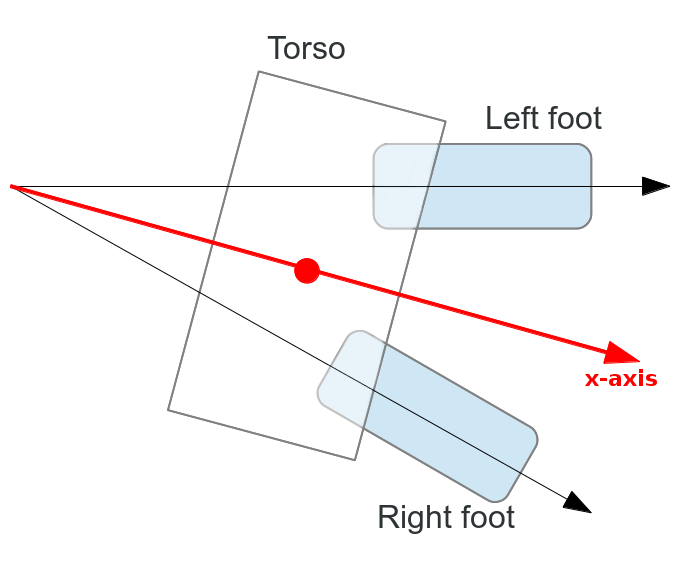
\includegraphics[width=0.48\textwidth]{img/sagittal_feet.png}
  \end{center}
  \vspace{-30pt}
  \caption{The sagittal $x$-axis is always defined as being forward from the IMU (or center of the torso). The neutral point (i.e. the origin) is the location of the IMU when the robot is in a standing pose, shown here as the red dot.}
  \label{fig:sagittal}
\end{figure}

Work was done on similar state measurement by Liu\cite{liu} through extensive filtering of the IMU's measurements. This had resulted in an inverted pendulum model which calculated a filtered angle for the torso lean. This filter remained in place for angular measurements. In order to maintain a relatively stable position state variable, a simple filter was used:

\begin{equation}
x^\star_t = \alpha * H\theta_t + (1 - \alpha) * H\theta_{t-1}
\end{equation}

For the filter, $x^\star_t$ is the filtered position state variable at time $t$, $H\theta_t$ is as in Equation~\ref{eq:simplified}, and $\alpha$ is a filtering rate between $0$ and $1$ (how much of the current measurement to use in the filter).

Attempts were made to also measure the state variables through integration of the accelerometer data, but, as the results in Section~\ref{sec:rl_results} show, these measurements were too unstable to be of any use.

\subsection{Generic Policy Interpreter}

As defined in Section~\ref{sec:learning_policies} and seen in Figure~\ref{fig:policy}, the reinforcement-learned control policies are output as a \textit{policy file} of $(\text{state-action}, \text{action})$ tuples. For the sake of generality, we will now refer to these as $(\text{state, action})$ pairs. The policy files are then parsed by the Nao's software during runtime initialisation and used as necessary for making decisions about actions to take. A simple parser and interpreter was used by White for the 2010 RL implementation. The work presented here is an improvement to White's implementation, as well as the application of the improved policies created by Hengst.

\subsubsection{Generic Policy File}

First, we define a generic policy file format as in Figure~\ref{fig:policy_def}:

\begin{figure}[h]
\newcommand\commenthigh[1]{\textcolor[rgb]{0,0.5,0}{#1}}
\begin{Verbatim}[commandchars=\\\{\},frame=single]
\commenthigh{// Comments are lines beginning with //}
\commenthigh{// The first non-comment line is the "resolution"}
   1     0.002   0.01  1
\commenthigh{// Each subsequent line defines a (state, action)}
\commenthigh{// goal  pos     vel  last    action}
   0    -0.080  -0.40  0        0
   0    -0.080  -0.39  1        1
   1    -0.080  -0.38  0        1
   1    -0.080  -0.37  1        2
\end{Verbatim}
\vspace{-15pt}
\caption{Definition of a policy file.}
\label{fig:policy_def}
\end{figure}

We define some terms:

\begin{description}
\item[State] -- A list of values defining a state. For the RL policy files, the state comprises the tuple of (goal, position, velocity, last action taken). These four values are defined as a possible ``state'' of the robot at any given time.
\item[Action] -- A single value of type \texttt{Action} which defines what action to take. The \textit{Action} type is defined in the codebase, and currently is simply an integer value.
\item[Comment] -- A line beginning with $//$ which is completely ignored by the parser.
\item[Resolution] -- This line contains exactly one number for every state variable. This number defines the exact distance between states for the respective state variable. In the example above, the third state variable (velocity) can only differ in steps of size $0.01$ exactly. Thus, $-0.40$ and $-0.39$ are valid velocity states, but $-0.395$ is not.
\end{description}


\subsubsection{RLPlanner}

On initialisation, the class parses a generic policy file and stores it in a lookup table. Depending on the resolution of the files, this may take up to several seconds per file.

A generic policy file is parsed by creating a map from states to an \texttt{Action} type. The  mappings are stored in a \verb!C++! \texttt{map<vector<int>, Action>} variable, essentially an $n$-dimensional lookup table, where $n$ is the number of state variables.

First, a vector of state variable resolutions is stored.

Next, each state is parsed. To allow for simpler state approximation and mapping lookup, each value is converted to an integer by dividing the resolution of the variable. For example, a value of $-0.39$ in a resolution of $0.01$ becomes the integer $-39$. The values of the state are stored as a single integer vector.


A simple interface function can be used to lookup an action from this table:

\begin{lstlisting}
// Get the next action given the state variables x1, x2, ..., xn
Action a = rlplanner->getAction(x1, x2, ..., xn);
\end{lstlisting}

The \texttt{getAction} function automatically rounds the state variables to the nearest state before performing the lookup.

\subsubsection{Using the RLPlanner}

A motion generator may use a policy file by creating an instance of the \texttt{RLPlanner} class.

A motion generator, such as \texttt{StandGenerator} (which defines the behaviour for standing upright and still), simply creates an instance of \texttt{RLPlanner} for each required policy file, then on every tick looks up an action to perform, and then performs it. The actions performed are those defined in Sections~\ref{sec:sagittal}~and~\ref{sec:coronal}.

\newpage
\section{Results}
\label{sec:rl_results}
Several policies were tested through the \texttt{StandGenerator} with mixed success. The sagittal standing still controller proved to be most successful and is described in more detail below. The similar coronal controller resulted in random oscillations of the robot due to the extra hip sway. These random oscillations sometimes diverged and quickly destabilised the robot, even with extremely heavy filtering of the gyrometer measurements. Due to a lack of reasonable results, the goals of rocking from foot to foot were not attempted.

Sagittal self-balancing control when standing still was found to be a significant improvement over no control policy. Upon being disturbed, the robot would actuate its hip motors and oscillate its body back into an upright position. When reacting to being pushed by human touch, the difference with and without the control policy could easily be felt, though it was somewhat more difficult to quantifiably verify. Simple tests were performed of releasing the robot from a certain lean angle with and without the control policy. The results of these tests can be seen in Table~\ref{tab:results} below, which shows a slight improved performance when using the control policy.

% TODO
\begin{table}[h]
  \centering
    \begin{tabular}{ r|c|c| }
    \multicolumn{1}{r}{}
     &  \multicolumn{1}{c}{no controller}
     & \multicolumn{1}{c}{sagittal controller} \\
    \cline{2-3}
    $5\degree$ &  &  \\
    \cline{2-3}
    $10\degree$ &  &  \\
    \cline{2-3}
    $15\degree$ &  &  \\
    \cline{2-3}
    $20\degree$ &  &  \\
    \cline{2-3}
    $25\degree$ &  &  \\
    \cline{2-3}
    $30\degree$ &  &  \\
    \cline{2-3}
    \end{tabular}
  \caption{Table of number of times robot was able to self-stabilise after being placed in a given sagittal angle.}
  \label{tab:results}
\end{table}

A minor point to be made was when the robot was in a standing still state, very tiny actuations still happened in the motors, causing a very small (basically imperceptible) oscillation of the torso back and forth. It is likely that this was caused by the significant noise apparent in the gyrometer measurements, and the constant actuation could potentially cause more wear on the motors than without the control policy.

The three-axis accelerometer was found to be too noisy to be of any significant use for any state measurements. While standing still, the accelerometer would report a large acceleration reading in the $z$-axis (as expected due to gravity), but also non-zero and wildly fluctuating accelerations in the $x$- and $y$-axes. Heavy filtering of these was found to be ineffective, as the offset from zero tended to drift randomly and in a non-Gaussian manner (making it difficult to filter). Integrating the non-Gaussian noise of course lead to a runaway velocity, which made the accelerometer unusable for measuring state.

Similar issues were observed with the gyrometers, which provided extremely noisy measurements. However, the gyrometers provided a somewhat more stable and accurate reading for the torso angle than the noisy accelerometers. The angle measurement was enough for the sagittal goal to work as mentioned above.

Despite the disappointing initial results, the work was presented at Robocup 2013 in The Netherlands for the Standard Platform League Open Challenge. The theoretical results of Hengst's work\cite{bernhard_rl} were described, a short video of simulated policies was shown (also by Hengst), and a the functioning standing policy was demonstrated against a robot with no control policy. rUNSWift's Open Challenge entry was awarded $3^{rd}$ place.

\newpage
\section{Future Work}

% TODO More complex state measurement

State measurement is currently the biggest obstacle to overcome. Finding a reliable and accurate way to measure the robot's body state is by far the biggest contributor to future stability work. More complex state measurement may involve the use of the Nao's joint position sensors to create a map of the robot's body in three-dimensional space, along with accelerometer and gyrometer data to determine attitude.

It is possible that simpler state measurement, such as tried in the work presented, may still allow for sufficient results through the use of more advanced filtering. The seemingly non-Gaussian nature of the noise in the sensors presented a challenge not able to be overcome by the author. However, as the results showed, even crude filtering could be used to some effect for the simpler stability problems like standing still.

It is quite likely that relying on the angle measurement of the torso for coronal policies is not suffcient. A potential theory for this may be the opposing forces of the hip sway on the ankle and hip joints acting to restore the torso to a zero angle but leaving the torso in a laterally displaced location. However, as the position state variable is calculated only based on torso angle, it's possible that the robot would assume it to be back in a neutral position in this case. Further investigation is required.

Further improvements can also be made to the generic policy file interpreter. Most importantly, sharing a single policy file between multiple generators is a function that should be added, as currently the system may read and store in memory the same policy file multiple times if called by multiple motion generators. No memory or performance issues were found during testing, but it is possible that large C++ maps may not be the most efficient structure for storage, and this should be further investigated if deemed necessary.

\section{Conclusions}
The work presented proves that control policies learned on simulations of the robots can be successfully used to perform self-stabilisation on the robots. This proves that the theory is sound and applicable to real-life hardware, and eventually applicable to more stable bipedal behaviours. A generic policy file format has been defined and an improved policy interpreter written. Both tools can be further improved for use in future exploration of RL applications.

Major failure points have been identified in state measurement. If the work presented here is to be expanded on, more must be done on improving the accuracy of measuring the robot's current position and velocity.
